\section{Experimental Setup}

\subsection{Noisy Annotations
Generation}\label{sec:noisy_annotations_generation}

A challenge arises for the creation of emulated noisy annotations datasets,
since it is expected for images annotations to have some degree of
expertise variability, similar to what is expected in real
crowdsourced datasets.
Simply introducing random noise into the annotated masks does not work,
since the original morphological structures from the expected ground
truth are far from being preserved. Instead, a ``noisy'' labeler is
expected to produce an annotation which has at least some degree of
morphological consistency on itself, even if it shows discrepancies
when compared with some metric (like DICE score) against the ground
truth annotation.

This has been proven experimentally when introducing random noise into any
popular segmentation dataset, in which the resulting mask is just a non
coherent map of noise across the image, as shown in Figure
\ref{fig:noisy_masks}.

\begin{figure}[h]
  \centering
  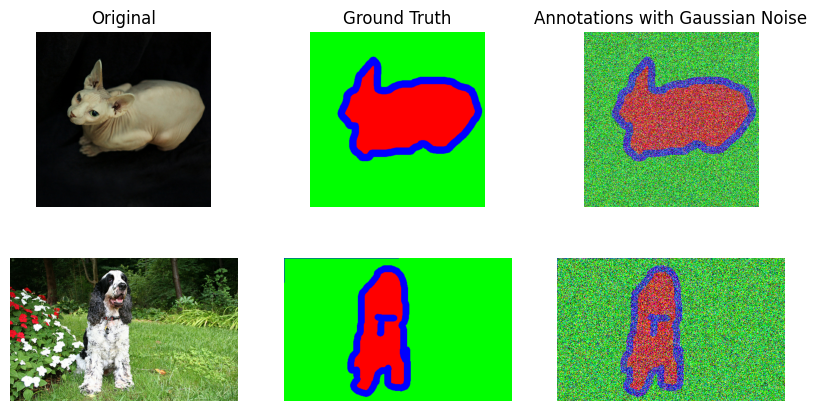
\includegraphics[width=0.7\textwidth]{Cap5/Figures/naive_gaussian_noise.png}
  \caption{Example of a noisy mask generated by naively introducing random
  noise into a ground truth mask. Morphological consistency is lost.}
  \label{fig:noisy_masks}
\end{figure}

For this reason, a more sophisticated approach was needed to create
datasets with emulated noisy annotations. The approach used here was
to use a pre-trained U-Net model to produce a good enough
\footnote{More precisely, a U-Net architecture with Resnet-34
  backbone model with a simple categorical cross-entropy loss which reached
$0.8426$ Dice Coefficient after 44 epochs.} segmentation of the
image, which was
then used to produce a ``noisy'' annotation by introducing random
noise into the last encoder layers of the model, thus preserving the
morphological consistency of the original annotation. This strategy
works since slight modifications introduced into the encoder layers
weights, resemble conceptual disturbances with respect to the
original ground truth label, which kind of emulates
the cultural behavior of having a different interpretation of the
image, either for having a different level of expertise or for having a
different point of view or school of thought. The first encoding layers
were not modified, since it is expected human labelers would agree on the
most fundamental structures (analog to extracted features from initial
convolutional layers) in a similar way, thus preserving some degree of
morphological consistency of the original annotation.

In this way, the level of ``disturbance'' with respect to the ground
truth for an emulated annotator can be controlled by the level of
noise introduced into the weights of the last encoder layers, thus:

\begin{equation}
  \mathbf{W}_{noisy} = \mathbf{W}_{original} + \epsilon_d
\end{equation}

where $\mathbf{W}_{original}$ represents the original weights of the
last encoder layers, $\epsilon_d$ follows a Gaussian distribution with
zero mean and variance $\sigma^2$. The variance $\sigma^2$ controls
the level of
noise introduced, and thus the degree of disturbance in the resulting
segmentation masks.

With the application of the encoder layer weight perturbation technique,
the resulting noisy masks are shown in Figure
\ref{fig:enhanced_disturbances}. It can be seen that the
morphological consistency is preserved, even though the resulting
masks are far from the ground truth annotations, which goes perfectly
well for testing the robustness of the models against noisy
annotations in crowdsourcing-like scenarios.
\begin{figure}[h]
  \centering
  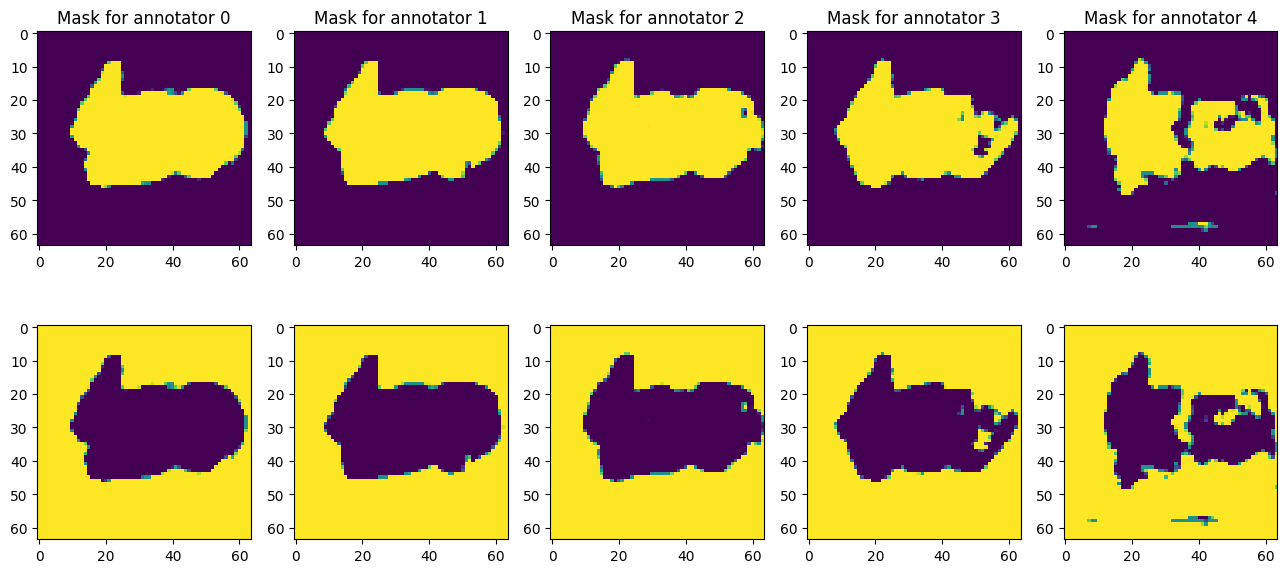
\includegraphics[width=0.8\textwidth]{Cap5/Figures/enhanced_disturbances.png}
  \caption{Noisy mask generated by enhancing the disturbances
    in the encoder layers weights for the Oxford-IIIT Pet Dataset.
    Morphological consistency is preserved. From left to right, SNR
    levels of noise in the encoder layer are 10, 5, 2, 0, -5 dB. Not
    adding noisy to the encoder layer would reach to an annotator
  behavior as good as the originally trained base model.}
  \label{fig:enhanced_disturbances}
\end{figure}

\subsection{Missing Labels Emulation}

It has also been determined that most real world crowdsourced datasets
suffer from missing labels, since not all annotators are able to label all
of the input samples. To emulate this behaviour, a missing labels dataset
was created by randomly skipping labels from the annotators labels
based on a labeling rate
$r_l \in [0, 1]$. The labeling rate $r_l$ controls the proportion of labels
that are skipped from the annotators labels. The lower the labeling rate,
the more labels are skipped from the annotators labels. The
implementation of this missing labels emulation
together with the noisy annotators generation can be flexibilized
through an algorithm, which enables it
to be used in experiments with variable amount of labelers, noise
levels, and labeling rates. An overview of the algorithm is shown in
Algorithm \ref{alg:multi_annotator_dataset_generation}. A sample of the
generated noisy and missing labels dataset is shown in Figure
\ref{fig:missing_labels_emulation}.

\begin{figure}[H]
  \centering
  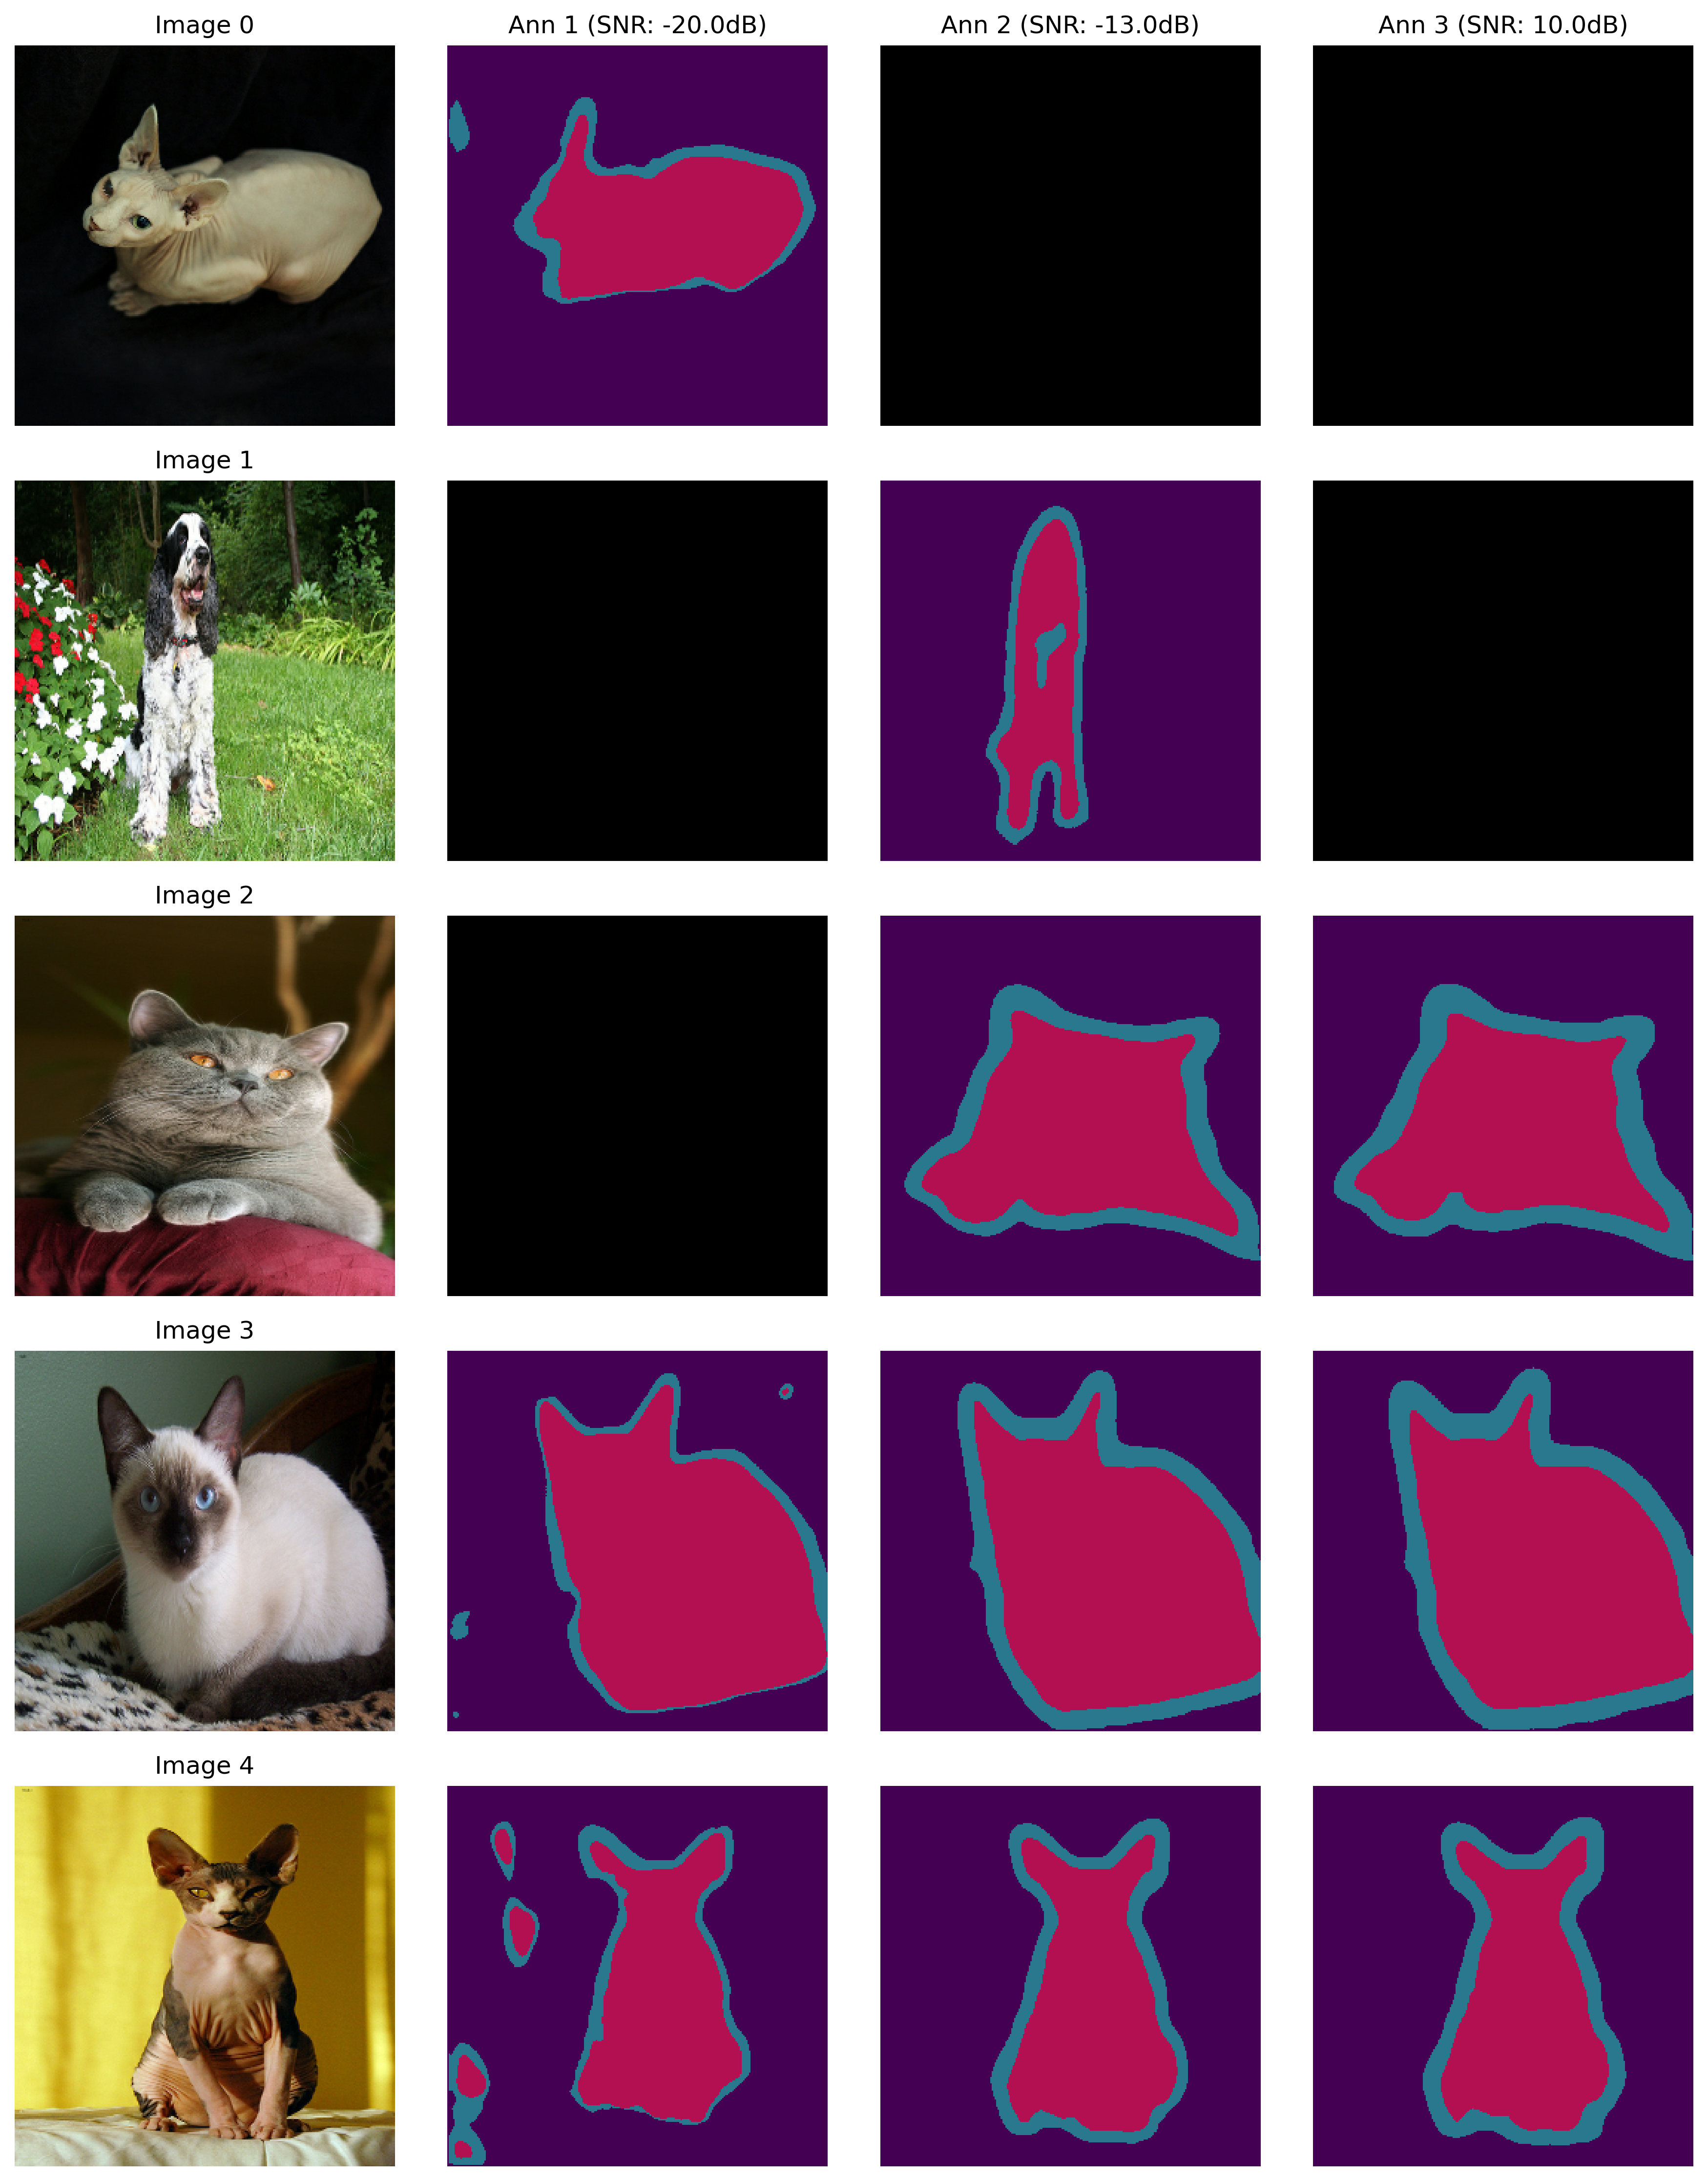
\includegraphics[width=0.7\textwidth]{Cap5/Figures/oxford_pet_missing_labels.png}
  \caption{Example of missing labels and noisy annotations emulation
    for the Oxford-IIIT Pet Dataset. The same label rate ($r_l =
    0.7$) is preserved for all labelers, which means in this case
    that every labeler is expected to label 70\% of the
  samples, and skip the remaining 30\%.}
  \label{fig:missing_labels_emulation}
\end{figure}

\begin{algorithm}
  \caption{Multi-Annotator Dataset Generation with Noisy and Missing Labels}
  \label{alg:multi_annotator_dataset_generation}
  \begin{algorithmic}[1]
    \Require Base segmentation model $M$, SNR levels $\{s_1, ...,
    s_n\}$, labeling rate $r \in [0,1]$
    \Ensure Dataset with multiple noisy annotations and missing labels

    \State \textbf{Step 1: Generate Noisy Annotators}
    \For{each SNR level $s_i$}
    \State Create disturbed model $M_i$ by adding noise to $M$
    with SNR $s_i$
    \EndFor

    \State \textbf{Step 2: Initialize Labeler Assignment System}
    \State Create assignment matrix $A \in \{0,1\}^{N \times n}$
    where $N$ is number of samples
    \For{each annotator $j \in \{1,...,n\}$}
    \For{each sample $i \in \{1,...,N\}$}
    \State $A_{i,j} \gets
    \begin{cases}
      1 & \text{with probability } r \\
      0 & \text{with probability } 1-r
    \end{cases}$
    \EndFor
    \EndFor

    \State \textbf{Step 3: Generate Multi-Annotator Dataset}
    \For{each image $x$ in dataset}
    \State Resize $x$ to target dimensions
    \For{each annotator model $M_i$}
    \State Generate annotation $y_i = M_i(x)$
    \State Apply labeler assignment mask: $y_i \gets y_i \cdot A_{i,j}$
    \EndFor
    \State Store $(x, \{y_1, ..., y_n\})$ in dataset
    \EndFor

    \Return Multi-annotator dataset with noisy and missing labels
  \end{algorithmic}
\end{algorithm}
